\chapter{Detailed Description}
\section{Interpreter}
The interpreter is a complete implementation of an interpreter for the -{}-C language. It accepts input from the parser in the form of an AST (\emph{Abstract Syntax Tree}) and obeys the instructions contained within the nodes of the tree. When given input as a tree, it is a fairly natural to approach to walk over this using some kind of tree walk and interpret on the fly. Hence, the main body of the interpreter is such a recursive tree walk. We will see this kind of recursive pattern several times throughout the whole project.
\ \\ \ \\
Firstly, the interpreter scans the AST, looking for global variables and function definitions. This initial scan is done, as we have no idea where to start interpreting without the presence of some kind of entry point into the user's code. It was decided that the most sensible approach would be to require the user-supplied definition of an \verb!int main(void)! entry-point function, in a similar vain to C. As this initial sweep of the AST takes place, any global variables or function declarations are entered into a structure known as the ``environment". Quite simply, the environment houses everything that the interpreter considers to be ``in-scope" at a given execution point. As such, after our initial scan, we can detect the presence of a valid entry-point function by examining the environment. This initial environment is known as the ``global environment", as everything contained within, is visible to the whole user programme. This initial scan follows exactly the same code-path as the full interpreter does, but passes a flag, in order to ensure that function bodies are never stepped into.
\ \\ \ \\
The environment (depicted in figure \ref{fig:environment}) is a hash-table of \verb!values!. These values are references to inner functions or local variables. By following the static link (see diagram), it is possible to see how values can be accessed from higher scopes. The idea of a static link was given to us in relation to their use in Activation Records (please see section \ref{section:MIPS}) during lectures. Different information is stored for functions as opposed to variables. The \verb1value1's type is determined with the following constants, the main types are given here, although there are some used for other purposes that are not mentioned here for the sake of clarity.

\begin{description}
	\item[VT\_INTEGR] Values of this type are integer variables, integer constants or integer temporaries.
	\item[VT\_STRING] Strings cannot be stored in the environment (this language does not have a string type), this value type is used to construct temporary strings that can be passed around within the interpreter / compiler. Such string values are created when identifiers are walked over, for instance.
	\item[VT\_FUNCTN] These values represent pointers to functions. This can be either a function variable or an actual function.
\end{description}

\ \\ \ \\
If no entry point is found, a fatal error is raised as interpretation cannot continue without a valid entry point. If the entry point was found in our global environment, we lookup where the function definition was found in the AST and execute from this point. The difference between this and the initial scan, is that we now look inside function bodies and any nested functions contained therein. Every time we enter a new function or block (such as an \emph{if statement} or \emph{while loop}), a new environment is created with a static link to the environment of the parent (enclosing) function (or the global environment, as appropriate).
\ \\ \ \\
As we step over the tree in this recursive function (\verb!evaluate!), we encounter \verb!NODES! that are present in the AST. The following steps are taken for the different types of node:

\begin{description}
	\item[Arithmetic Operator] We look at the LHS of the expression and the RHS and call evaluate recursively on each. From each recursive call we get back a \verb!value! typed struct for each. This will be the integer value on the LHS and RHS. If one side happened to be a function application, for instance, the recursive call has already made the necessary calls to simplify this to an integer value. We calculate the result of the arithmetic expression and return the appropriate value.
	
\end{description}


\begin{figure}[p]
	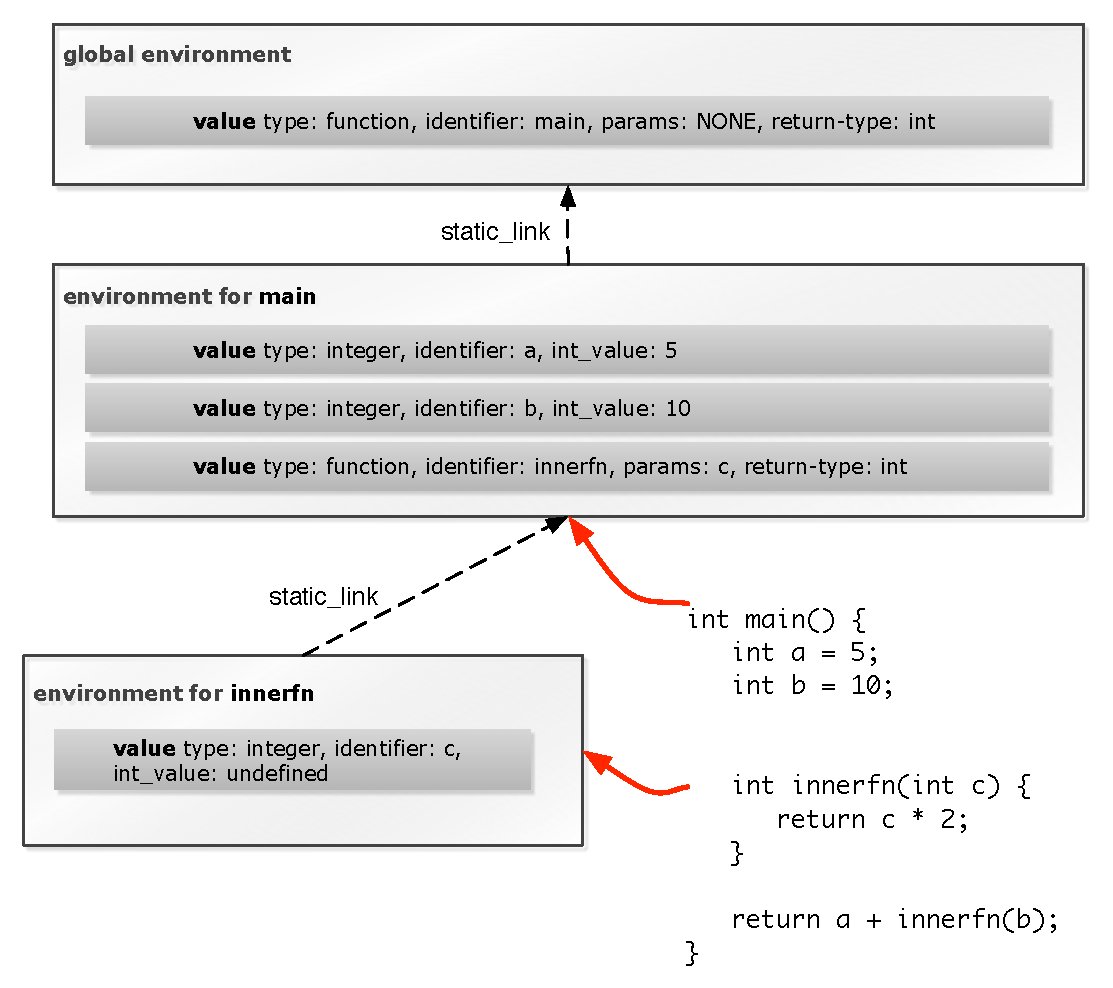
\includegraphics[scale=0.7]{environments-include.pdf}
	\label{fig:environment}
	\caption{Environment Layout - Environment $\rightarrow$ Code relationship}
\end{figure}


\section{Intermediate Representation}
\label{section:MIPS}
\section{MIPS Assembler Compiler}